\documentclass[main.tex,fontsize=8pt,paper=a4,paper=landscape,DIV=calc,]{scrartcl}
% Document
\usepackage[T1]{fontenc}
\usepackage[utf8]{inputenc}
\usepackage[dvipsnames]{xcolor}
\usepackage[nswissgerman,english]{babel} 
\usepackage{hyperref}
\renewcommand{\familydefault}{\sfdefault}

% Format
\usepackage[top=5mm,bottom=5mm,left=5mm,right=5mm]{geometry}
%\setlength{\headheight}{\baselineskip}
%\setlength{\headsep}{0mm}

%\usepackage{scrlayer-scrpage}
%\clearpairofpagestyles
%\chead{{\bfseries\TITLE, \AUTHOR, \pagename~\thepage}}

%\addtokomafont{pagehead}{\upshape}

\usepackage{multicol}
\setlength{\columnsep}{2mm}
\setlength{\columnseprule}{0.1pt}

% Math
\usepackage{amsmath}
\usepackage{amssymb}
\usepackage{amsfonts}

% Code
\usepackage{fancyvrb, etoolbox, listings, xcolor}
%\usemintedstyle{bw}

%\newminted[shell]{bash}{
%fontsize=\footnotesize,
%fontfamily=tt,
%breaklines=true,
%frame=single,
%framerule=0.1pt,
%framesep=2mm,
%tabsize=2
%}
%\newminted{css}{
%breaklines=true,
%tabsize=4,
%autogobble=true,
%escapeinside=||,
%stripall=true,
%stripnl=true,
%}

    \definecolor{lightgray}{rgb}{0.95, 0.95, 0.95}
    \definecolor{darkgray}{rgb}{0.4, 0.4, 0.4}
    \definecolor{purple}{rgb}{0.65, 0.12, 0.82}
    \definecolor{ocherCode}{rgb}{1, 0.5, 0} % #FF7F00 -> rgb(239, 169, 0)
    \definecolor{blueCode}{rgb}{0, 0, 0.93} % #0000EE -> rgb(0, 0, 238)
    \definecolor{greenCode}{rgb}{0, 0.6, 0} % #009900 -> rgb(0, 153, 0)
    \definecolor{teal}{rgb}{0.0, 0.5, 0.5}

\lstdefinestyle{code}{
    identifierstyle=\color{black},
    keywordstyle=\color{blue}\bfseries\small,
    ndkeywordstyle=\color{greenCode}\bfseries\small,
    stringstyle=\color{ocherCode}\ttfamily\small,
    commentstyle=\color{teal}\ttfamily\textit\small,
    basicstyle=\ttfamily\small,
    breakatwhitespace=false,         
    breaklines=true,                 
    captionpos=b,                    
    keepspaces=true,                 
    showspaces=false,                
    showstringspaces=false,
    showtabs=false,                  
    tabsize=2,
    belowskip=-5pt
}



% Images
\usepackage{graphicx}
\newcommand{\pic}{\includegraphics[scale=0.3]}
\graphicspath{{Screenshots/}{../Screenshots}}
\makeatletter
\def\pictext#1#2{%
    \@ifnextchar[{%
    \pictext@iiiii{#1}{#2}%
    }{%
      \pictext@iiiii{#1}{#2}[0.5,0.4,0.3]% Default is 5
    }%
}
\def\pictext@iiiii#1#2[#3,#4,#5]{\begin{minipage}{#3\textwidth}\includegraphics[scale=#4]{#1}\end{minipage}\begin{minipage}{#5\textwidth}#2\end{minipage}}
\def\minipg#1#2{%
    \@ifnextchar[{%
    \minipg@iiii{#1}{#2}%
    }{%
      \minipg@iiii{#1}{#2}[0.3,0.6]% Default is 5
    }%
}
\def\minipg@iiii#1#2[#3,#4]{\vspace{0.8mm}\begin{minipage}{#3\textwidth}#1\end{minipage}\begin{minipage}{#4\textwidth}#2\end{minipage}{\vspace{0.8mm}}}
\makeatother

%\newenvironment{minty}[2]% environment name
%{% begin code
%  \begin{minipage}{#1}
%  \begin{minted}{#2}
%}%
%{% end code
%  \end{minted}
%  \end{minipage}
%  \end{minty}\ignorespacesafterend
%} 

% Smaller Lists
\usepackage{enumitem}
\setlist[itemize,enumerate]{leftmargin=3mm, labelindent=0mm, labelwidth=1mm, labelsep=1mm, nosep}
\setlist[description]{leftmargin=0mm, nosep}
\setlength{\parindent}{0cm}

% Smaller Titles
\usepackage[explicit]{titlesec}

%% Color Boxes
\newcommand{\sectioncolor}[1]{\colorbox{black!60}{\parbox{0.97\linewidth}{\color{white}#1}}}
\newcommand{\subsectioncolor}[1]{\colorbox{black!50}{\parbox{0.97\linewidth}{\color{white}#1}}}
\newcommand{\subsubsectioncolor}[1]{\colorbox{black!40}{\parbox{0.97\linewidth}{\color{white}#1}}}
\newcommand{\paragraphcolor}[1]{\colorbox{black!30}{\parbox{0.97\linewidth}{\color{white}#1}}}
\newcommand{\subparagraphcolor}[1]{\colorbox{black!20}{\parbox{0.97\linewidth}{\color{white}#1}}}

%% Title Format
\titleformat{\section}{\vspace{0.3mm}\bfseries}{}{0mm}{\sectioncolor{\thesection~#1}}[{\vspace{0.3mm}}]
\titleformat{\subsection}{\vspace{0.3mm}\bfseries}{}{0mm}{\subsectioncolor{\thesubsection~#1}}[{\vspace{0.3mm}}]
\titleformat{\subsubsection}{\vspace{0.3mm}\bfseries}{}{0mm}{\subsubsectioncolor{\thesubsubsection~#1}}[{\vspace{0.3mm}}]
\titleformat{\paragraph}{\vspace{0.3mm}\bfseries}{}{0mm}{\paragraphcolor{\theparagraph~#1}}[{\vspace{0.3mm}}]
\titleformat{\subparagraph}{\vspace{0.3mm}\bfseries}{}{0mm}{\subparagraphcolor{\thesubparagraph~#1}}[{\vspace{0.3mm}}]

%% Title Spacing
\titlespacing{\section}{0mm}{0mm}{0mm}
\titlespacing{\subsection}{0mm}{0mm}{0mm}
\titlespacing{\subsubsection}{0mm}{0mm}{0mm}
\titlespacing{\paragraph}{0mm}{0mm}{0mm}
\titlespacing{\subparagraph}{0mm}{0mm}{0mm}

%% format cells
\usepackage[document]{ragged2e}
\usepackage{array, makecell}
\renewcommand{\arraystretch}{2}
\newcommand{\mc}{\makecell[{{m{1\linewidth}}}]}



\begin{document}
\begin{multicols*}{4}

\lstset{
    language={[x86masm]Assembler},
    style=code,
}

\section{Assembly}
Assembly is a platform -> intel, arm, risc-v dependent programming language. 
It converts instructions into binary -> machine code. Most compiled language will convert to assembly code before being compiled to binary!

\subsection{Numbers in Assembly}
\begin{itemize}
\item \textcolor{black}{db 48 -> Byte 48d}
\item \textcolor{black}{db 0x35, 0h21, 049h -> Bytes 35h, 21h, 49h}
\item \textcolor{black}{db 'a' -> ASCII-Code a == 61h == db 0x61}
\item \textcolor{purple}{db == Byte -> 8 Bit}
\item \textcolor{purple}{dw == Word -> 16 Bit == db first-nr, db second-nr}
\item \textcolor{purple}{dd == Doubleword -> 32 Bit}
\item \textcolor{purple}{dq == QuadWord -> 64 Bit}
\item \textcolor{orange}{048d -> d for decimal}
\item \textcolor{orange}{048h or 0x48 -> h for hex}
\item \textcolor{orange}{10001000b or 1000\_1000b -> b/y for binary}
\end{itemize}
\subsection{Length Calculation}
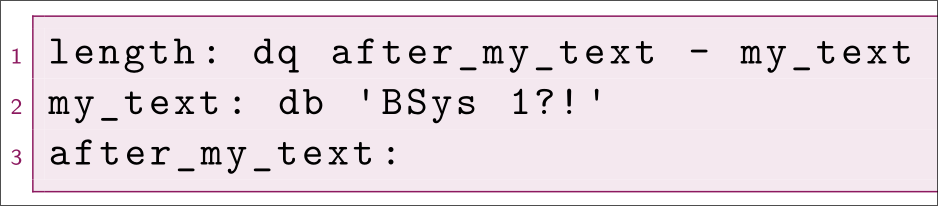
\includegraphics[scale=0.2]{2022-09-27-04_27_52.png}
first define a quadword with 2 unknown labels, then define my\_text with 'Besys',
after define aftermytext and recude the current instruction pointer with the instruction pointer at my\_text
\subsection{Default Registers}
\begin{itemize}
\item Right 8 bit register: \textcolor{purple}{AL}
\item Left 8 bit register: \textcolor{purple}{AH}
\item 16 bit register: \textcolor{purple}{AX}
\item 32 bit register: \textcolor{purple}{EAX}
\item 64 bit register: \textcolor{purple}{RAX}
\end{itemize} 

\subsection{Special Registers}
\begin{itemize}
  \item \textcolor{purple}{RAX} general use register
  \item \textcolor{purple}{RCX} Counter for loops or strings
  \item \textcolor{purple}{RDX} Pointer for I/O Operations
  \item \textcolor{purple}{RBX} Datapointer
  \item \textcolor{purple}{RSI,RDI} Source for stringoperations
  \item \textcolor{purple}{RSP} Stackpointer!!
  \item \textcolor{purple}{RBP} Basepointer
  \item \textcolor{purple}{R8-R15} additional registers
\end{itemize}
Note other registers like RBX exist as well, but aren't specifically used for something.

\subsection{Dealing with Memoryi}
Memory is accessed with the [] operators, this can also be offset with either multiplication or other calulations
\vspace{-2.5mm}
\begin{lstlisting}
mov rax, [0x8000] ; ok move 8000h into rax
mov [0x8000], rax ; ok move value at rax into 0x8000
mov rax, rbx      ; ok move rbx into rax, no memory access!!
mov [0x8000], [0x7000] ; error can't move memory to memory!!
\end{lstlisting}
\vspace{2mm}

\subsection{Assembly Instructions}
\begin{itemize}
\item mov rax, 1 \textcolor{teal}{//move the value 1 into rax, keep in mind that mov can hold other operations!}
\item equ rax, 1+1 \textcolor{teal}{//arithmic operation}
\item add z,   q  \textcolor{teal}{// z + q} 
\item sub z,   q  \textcolor{teal}{// z - q}
\item adc z,   q  \textcolor{teal}{// z + q + c (carry -> previous calculation)}
\item sbb z,   q  \textcolor{teal}{// z - q - c (carry -> previous calculation)}
\item neg z       \textcolor{teal}{// 0 - z ("zweierkomplement")}
\item inc z       \textcolor{teal}{// z++ }
\item dec z       \textcolor{teal}{// z-- }
\item mul z,      \textcolor{teal}{// multiply with implicit 2.operand }\newline
mul rbx -> RDX:RAX <-- RAX * RBX
\item imul z,   i  \textcolor{teal}{// signed equivalent for mul, z * i }
\item div z,      \textcolor{teal}{// divide with implicit 2.operand}\newline
div rbx  \newline
d = RDX:RAX\newline
RAX <-- RDX:RAX / RBX\newline
RDX <-- RDX:RAX mod RBX
\item shl z,   i  \textcolor{teal}{// z * \(2^i\)               --> shift}
\item shr z,   i  \textcolor{teal}{// z * \(2^{-i}\) z signed   --> shift}
\item sar z,   i  \textcolor{teal}{// z * \(2^{-i}\) z unsigned --> shift}
\item rol z,   i  \textcolor{teal}{// Left-Rotate i Bits }
\item ror z,   i  \textcolor{teal}{// Right-Rotate i Bits }
\item and rax, rbx\textcolor{teal}{// AND}
\item not rax     \textcolor{teal}{// NOT}
\item test rax, rax \textcolor{teal}{// set ZF = 1 if rax == 0}
\item jmp S       \textcolor{teal}{// Jump to S > GOTO}
\item cmp rax, 3 \textcolor{teal}{// compare rax and 3, set ZF = 1 if not}
\item cmov rax, 5 \textcolor{teal}{// move 5 into rax if condition met}
\item je 230 \textcolor{teal}{// move 230 down if condition met}
\item push rax \textcolor{teal}{// push rax to the stack}\newline
  sub rsp, 8 AND mov [rsp], rax \textcolor{teal}{stack pointer down}
\item pop rax \textcolor{teal}{// pop rax from the stack}\newline
  mov rax, [rsp] AND add rsp, 8 \textcolor{teal}{stack pointer up}
\item call S \textcolor{teal}{// push rax and jmp S > function call}
\item ret    \textcolor{teal}{// pop rax and jmp rax > return}
\end{itemize}

\subsubsection{Stack}
Note that the stack has the highest address from the bottom, meaning that adding to the stack decreases the stack pointer (rsp)!!

\subsubsection{Flags}
\textcolor{purple}{Carry Flag (CF) == overflow with unsigned intergers}\newline
0000 + 1111 = 0000, CF = 1 --> 1 + 15 = 0, CF = 1
\textcolor{purple}{OverFlow Flag (OF) == overflow with signed integers}\newline
0011 + 0001 = 1000 -> 7 + 1 = -8 (negative prefix)
\textcolor{purple}{Zero Flag (ZF) == set when result is 0}
\textcolor{purple}{Sign Flag == is the highest bit of the result}
\textcolor{purple}{Parity Flag (PF) == set if lowest bute has an even number of bits}

\subsubsection{Usage of compare with Condition Codes}
\textcolor{teal}{A : Above } \textcolor{teal}{ -> CF = 0 AND ZF = 0}\newline
\textcolor{teal}{AE: Above or Equal } \textcolor{teal}{ -> CF = 0}\newline
\textcolor{teal}{B : Below } \textcolor{teal}{ -> CF = 1}\newline
\textcolor{teal}{BE: Below or Equal } \textcolor{teal}{ -> CF = 1 AND ZF = 1}\newline
\textcolor{teal}{E : Equal } \textcolor{teal}{ -> ZF = 1}\newline
\textcolor{teal}{G : Greater } \textcolor{teal}{ -> SF = OF = 0 AND ZF = 0}\newline
\textcolor{teal}{GE: Greater or Equal } \textcolor{teal}{ -> SF = OF}\newline
\textcolor{teal}{L : Less } \textcolor{teal}{ -> SF != OF}\newline
\textcolor{teal}{LE: Less or Equal } \textcolor{teal}{ -> SF != OF AND ZF = 1}\newline
\textcolor{teal}{PE: Parity Even}  \textcolor{teal}{ -> PF =1}\newline
\textcolor{teal}{PO: Parity Old } \textcolor{teal}{ -> PF = 0}\newline
\textcolor{teal}{Z:  Zero} \textcolor{teal}{ -> ZF = 1}

\subsection{Syscall}
Syscalls are special operations that the Operating system understands
\vspace{-2.5mm}
\begin{lstlisting}
mov rax, 60 // 60 == exit instruction
mov rdi, 0 // exit code -> 0 means ok
syscall // OS executes instruction from rax
\end{lstlisting}
\vspace{2mm}

\subsection{Frame Pointer}
This is used to get a static point from where you can get your parameters from, as the stack pointer moves around!
\vspace{-2.5mm}
\begin{lstlisting}
; Prolog: create frame pointer
push rpb ;push base pointer to stack
mov rbp, rsp ;rsp into rpb
; Epilog: remove frame pointer
mov rsp, rpb ; move rpb into rsp 
pop rbp ; pop rbp from stack
\end{lstlisting}
\vspace{2mm}


\lstset{
    language=c,
    style=code,
}
\section{C}
Preprocessor -> Compiler -> Assembler -> Linker

\subsection{Precprocessor Tokens}
\begin{itemize}
\item \textcolor{purple}{Identifier}\newline
starts with a-z, A-Z followed by letters, digits or \_
\item \textcolor{purple}{Precrocessor Number}\newline
  starts with a digits followed by digits, numbers, \_, ., or exponents
\item \textcolor{purple}{String or Character literals}\newline
  string starts with ", char with ', escape \textbackslash 
\item \textcolor{purple}{Operations and punctuators}\newline
  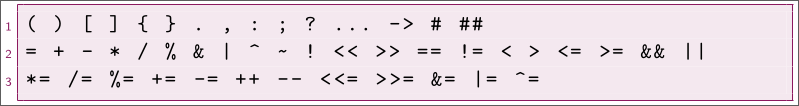
\includegraphics[scale=0.24]{2022-10-11-03_40_12.png}
\item \textcolor{purple}{others}
\end{itemize} 

\textbf{1. Iteration, removes all comments, 2. iteration, converts code to tokens, 3.iteration replaces macros with code}

\subsection{sizeof(t)}
\vspace{-2.5mm}
\begin{lstlisting}
// size of types, architecture dependent!
int a = 5;
printf("&d",sizeof(a)); // 16 for intel x86
\end{lstlisting}
\vspace{2mm}
\textcolor{red}{Note the return type is \textbf{size\_t} which is big enough to hold any type}

\subsection{Pointers}
\vspace{-2.5mm}
\begin{lstlisting}
int a = 5;
int *b = &a; // b pointer to a 
a = *b + 5; // a = dereference b and add 5
\end{lstlisting}
\vspace{2mm}
\textcolor{teal}{Incrementing a pointer will skip \textbf{sizeof(t) bytes!}}
\textcolor{orange}{Check for nullptr with ptr == 0 as c has no nullptr!}
Note, C has no references, that is a c++ thing

\subsection{Numbers in C}
\begin{itemize}
\item \textcolor{teal}{Decimal: 0..9 with \textbf{NO 0 at the start}}
\item \textcolor{teal}{Octal: 0..7 with a \textbf{leading 0}}
\item \textcolor{teal}{Hex: 0..F with \textbf{leading 0x}}
\item \textcolor{teal}{Suffix: the suffic specifies a type:}\newline
  l: long, ll: long long, u: unsigned, ul: unsigned long, ull ....
\end{itemize} 

\subsection{Bitwise Operators}
\textcolor{teal}{not: \(\tilde{} \) q} | \textcolor{teal}{and: q \& p} | \textcolor{teal}{or: q | p} \newline
\textcolor{teal}{left shift: q << p} | \textcolor{teal}{right shift: q >> p}

\subsection{Arithmic Operators}
like c++, \textcolor{red}{BUT RETURN TYPE IS INTEGER!!!!!}

\subsection{Parameters in Functions}
In C, you can pass any amount of parameters to a function, as long as the parameter type is not void:
\vspace{-2.5mm}
\begin{lstlisting}
void f () ;
void b ( void ) ;
// formatting to keep the lines shorter
void f() { printf("pangping!"); } // ok
void f(1, 2, 3, 4) { ... } // ok LMAO
void b() { ... } // ok
void b(1, 2, 3, 4) { ... } // !! ERROR !!
\end{lstlisting}
\vspace{2mm}

\subsection{Global vs Local}
Global variables are allocated on the heap, therefore they receive a default value -> int to 0, local variables are on stack -> undefined behavior by default

\subsection{printf Identifiers -> Strings! "\%d"}
\begin{itemize}
\item \textcolor{teal}{sizeof(Integer) as signed decimal = \%d}
\item \textcolor{teal}{sizeof(Integer) as unsigned decimal = \%u}
\item \textcolor{teal}{sizeof(Integer) as hexadecimal = \%x or \%U}
\item \textcolor{teal}{sizeof(long) as signed decimal = \%li}
\item \textcolor{teal}{sizeof(long long) as signed decimal = \%lli}
\item \textcolor{teal}{sizeof(void *) as pointer = \%p}
\item \textcolor{teal}{sizeof(char *) as pointer (null terminated) = \%s}
\item \textcolor{teal}{sizeof(double) as floating point = \%f}
\end{itemize}

\subsection{typedef}
\vspace{-2.5mm}
\begin{lstlisting}
typedef int int32_t // int as 32 bit int 
typedef int (* func) ( param )
// function as integer type
\end{lstlisting}
\vspace{2mm}

\subsection{Strings in C}
Strings in C are not 0 terminated, meaning you have to do it yourself!
They are just \textbf{char arrays!!}

\subsection{Const}
There is no proper const in C, there is only the let equivalent in rust, where the underlying variable is not mutable, but other fucntion can mutate the said value of the variable!!

\subsection{extern}
The extern symbol in C are meant for variables that are defined in another file, it is therefore not a declaration nor an initialization!

\subsection{static}
Static variables are essentially hidden global variables, meaning that they will never go out of scope until the program ends, but they can't be accessed outside of the scope!These values are default initialized, as they are syntactic sugar for global variables!

\subsection{Structs}
\vspace{-2.5mm}
\begin{lstlisting}
struct something { int q; // ... };
struct something fun = {5};
// struct keyword + struct name + variable name
// or nameless with struct { int q; } fun;
// access with fun.q or with pointers fun->q
\end{lstlisting}
\vspace{2mm}

\subsection{Unions}
\textcolor{red}{Unions point to the same memory, meaning that you can have multiple members that will point to a certain memory location and you can interpret them all at once! The size is determined by the biggest member}
\vspace{-2.5mm}
\begin{lstlisting}
typedef union U { int_64 first; char bytes[8]; } U;
U test;
test.first = 17;
// bytes == 11 00 00 00 00 00 00 00 == 17!!
\end{lstlisting}
\vspace{2mm}

\subsection{Complete vs Incomplete}
Complete types are of known size at compile time, incomplete types are not, they are therefore heap allocated!

\subsection{Malloc and free}
\vspace{-2.5mm}
\begin{lstlisting}
some_type *pointer = 0;
void initialize() {
  size_t count = 5;
  pointer = malloc(count * sizeof(some_type));
  // rest of the program 
  free(pointer);
  pointer = 0; // reset to prevent segfault
}
\end{lstlisting}
\vspace{2mm}

\section{Cache}

\subsection{Locality Principle}
This is the reason for L1,L2,L3 cache, the closer the cache is to the cpu, the less the data needs to travel, this can affect latency in todays hardware!

\subsection{Median Access Time}
\textcolor{red}{\(E(T) = P_C * T_C + (1 - P_C )* T_M\)}\newline
\(T_C\): Access time on Cache |
\(T_M\): Access time on Memory |
\(P_C\): Probability of Cache-Hit, likely above 0.9

\subsection{Fully Associative Cache FAC}
Every Byte OR Cacheline is mapped to 1 address on the cache. If full, new entry deletes an old entry.
\textcolor{red}{Costs a lot, one lookup part per entry!!}, \textcolor{green}{Really fast}

\subsection{Cacheline}
Instead of storing every byte, we can store 64 bytes as one. \textcolor{red}{Because every 64 bytes has the last 6 bits as 0, we can use these as an offset to indicate which byte we want to access!!}
\textcolor{purple}{Calculation for 6 bit offset: 84480801h / \(2^6\) = 8448080h / \(2^2\) = 2112020h, offset = 1 }

\subsection{Direct Mapped Cache DMC}
This stores each block in a specific cacheline. 
It does this by indexing each cacheline with bits. The amount needed for this is called \textbf{p}. 
We can split the address now even further into \textbf{reduced tag and line number}.
For the next example, consider the amount of cachelines to be 8.
\textcolor{purple}{Calculation for tag and linenumber: 2112020h / \(2^p\) => tag:21120, linenumber:20, offset:1}
\textcolor{red}{Now you only need one comparator for the tag, as the rest is already stored in a fixed position!!}\newline
\textcolor{OliveGreen}{Note that tag 52315, linenumber: 20 would be stored at the same place!}

\subsection{k-Way Set-Associative-Cache SAC}
\textcolor{purple}{One DMC per "Way". Best compromise between both.}\newline
k defines the amount of DMC used. 
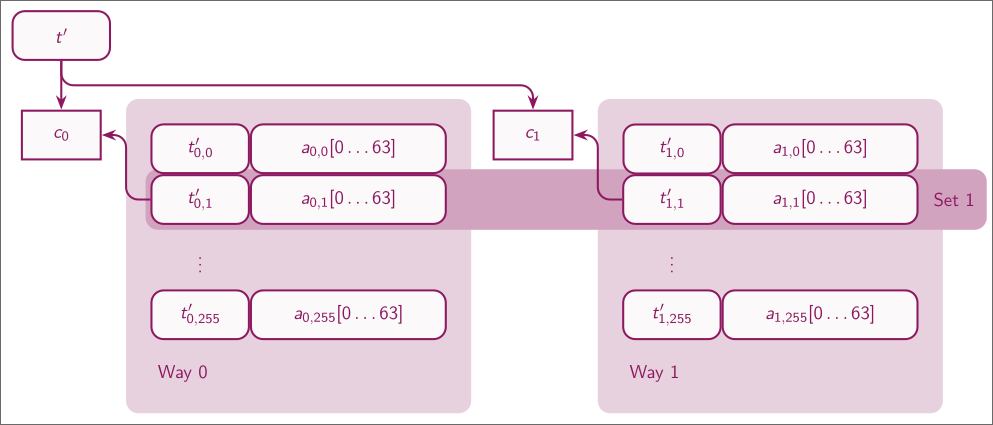
\includegraphics[scale=0.2]{2022-12-27_01_42_01.png} 
\textcolor{red}{Solves the issue of collisions from the DMC!}

\section{Fragmentation}
\textcolor{OliveGreen}{Internal Fragmentation:} Process wants 5 Bytes, but receives 200 due to system. \newline
\textcolor{OliveGreen}{External Fragmentation:} Process frees memory that can cause blocks of unallocated memory that aren't necessarily useful

\subsection{Search Algorithm}
\begin{itemize}
\item \textcolor{purple}{First Fit}
\item \textcolor{purple}{Next Fit} first AFTER last reserved!
\item \textcolor{purple}{Best Fit} smallest possible
\item \textcolor{purple}{Worst Fit} biggest possible
\item \textcolor{purple}{Quick Fit} \newline
  first smallest element out of a list
\item \textcolor{purple}{Random Fit}
\end{itemize} 

\subsection{Buddy System}
Starts with the entire memory and splits down to smalles possible size.\newline
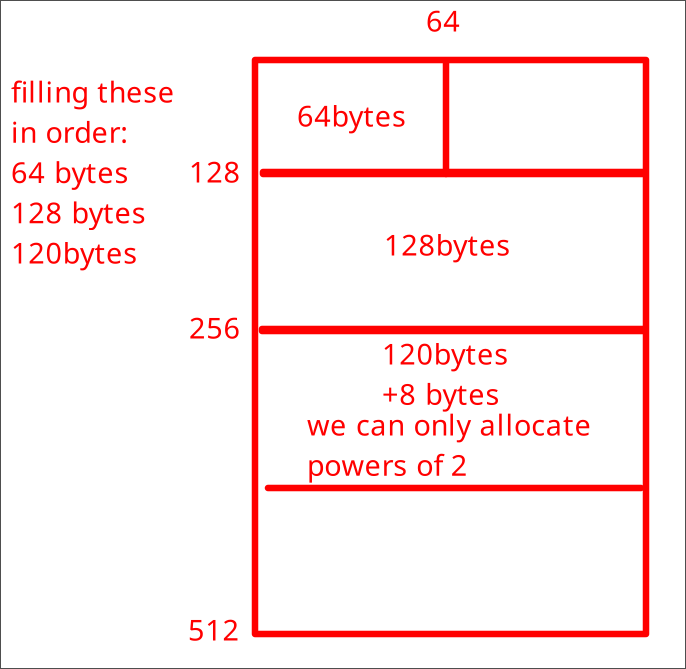
\includegraphics[scale=0.15]{2022-11-29-05_19_44.png}

\subsection{Object-Pools}
\begin{itemize}
\item \textcolor{purple}{Entire Memory split into equal sized objects}
\item \textcolor{purple}{No recombination, objects stay as they are}
\item \textcolor{purple}{if new objects are needed, new page is created}
\item \textcolor{purple}{Free objects stored in list}
\item \textcolor{purple}{Usually found in kernels}
\end{itemize} 

\subsection{Allocation in PenguinOS}
\textcolor{purple}{Buddy-System for big allocations (smallest size = 4kB), Object-Pool for kernel: \newline 
\textbf{SLAB,SLOB,SLUB::old,embedded,standard.}}

\subsection{Allocation in WinDoof}
\textcolor{orange}{FreeList[128]} stores free space, and is an array of pointers with size 128\newline
Additional Bitmap and cache over FreeList for fast lookup.\newline
Extra Cache over Bitmap for fast lookup on free space.\newline
Program chan choose between \textbf{Look-Aside List and Low-Fragmentation Heap implementation}\newline
Frontend commands: \textcolor{purple}{HeapCreate, HeapAlloc, HeapFree}\newline
HeapCreate chooses heap variant itself.

\section{RAM}
\textcolor{red}{Should access be invalid, then OS will throw segfault!}

\subsection{Terminology}
page = block of memory in storage
frame/block = block of memory in RAM
cacheline = block of memory in RAM
\textcolor{red}{ALL OF THESE HAVE THE SAME SIZE!}

\subsection{Pages}

\subsection{Memory Management Unit MMU}
The MMU maps physical RAM to virtual RAM via \textbf{Page-Table}.\newline
\textcolor{red}{One Page table per Process!}

\subsection{Translation Lookaside Buffer TLB}
\textcolor{purple}{Special Cache for MMU that only stores mappings}

\subsubsection{Page-Tables}
Page Tables can have multiple levels just like k-Way SAC.\newline
The root part of this is associated with a process.\newline
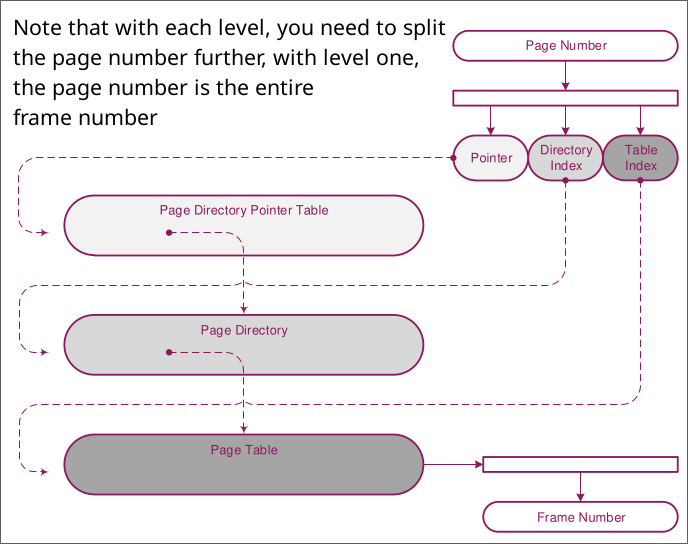
\includegraphics[scale=0.27]{2022-12-06-04_46_09.png}\newline
\textcolor{red}{Page-Tables always allocate the entire list! Page Directories only allocate the entries when they exist!}\newline
This is because you always need the space for the actual entry, but you don't need the space for an abstraction!
\textcolor{teal}{There are other implementations like Inverted Page Table or Hash Page Table, but they are not used}

\subsection{Interrupt}
MMU will throw interrupts, which the OS needs to handle.\newline
For example when an address is not in physical memory!\newline

\subsection{Status, Access and Dirty Bit}
\begin{itemize}
\item \textcolor{black}{S=1} -> Page in physical RAM
\item \textcolor{black}{A=1, D=0} -> recently read
\item \textcolor{black}{A=1, D=1} -> recently written
\item \textcolor{black}{A=0, D=1} -> written a while ago
\item \textcolor{black}{A=0, D=0} -> there was no access for a while
\end{itemize}
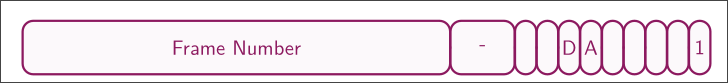
\includegraphics[scale=0.27]{2022-12-13-03_22_16.png}

\subsection{Paging Strategies}
Consists of \textcolor{purple}{Fetching Policies, Cleaning Policies and Replacement Policies} 

\subsection{Fetching Policies | loading from storage}
\begin{itemize}
\item \textcolor{purple}{Demand Paging} low effort, slow
\item \textcolor{purple}{Prepaging} preload based on guess
\item \textcolor{purple}{Demand Paging with Prepaging}\newline
  Like demand but loads neighbours as well
\item \textcolor{purple}{Increasing based on Heuristics}
\end{itemize} 

\subsection{Cleaning Strategies | writing to storage}
\begin{itemize}
\item \textcolor{purple}{Demand Cleaning} low effort, slow
\item \textcolor{purple}{PreCleaning or Page Buffering} Write on guess
\end{itemize} 

\subsection{Replacement Strategies | both at once}
Obvious ones: \textbf{\textcolor{purple}{FIFO, NFU without aging(not used), Best (not realistic, future known..)}}
\subsubsection{Second Chance / Clock}
Chain like FIFO with the A-bit being checked.\newline
\textbf{If A-Bit is set, then don't drop page, instead add page to the back and set A-bit to 0}, if \textbf{A-bit not set, drop page}\newline
\textcolor{purple}{Clock is a more efficient version where only pointer moves, circular movement!}\newline

\subsubsection{Least Recently Used LRU}
Replace page that has not been used for the longest time.\newline
\textcolor{purple}{Time noted on each MMU access, requires compatible MMU}

\subsubsection{Not Frequently Used with Aging NFU}
OS creates interval, if MMU accesses page within interval, counter increases.\newline
\textcolor{red}{Counter is binary! With each iteration, counter is shifted to right (aging!)}\newline
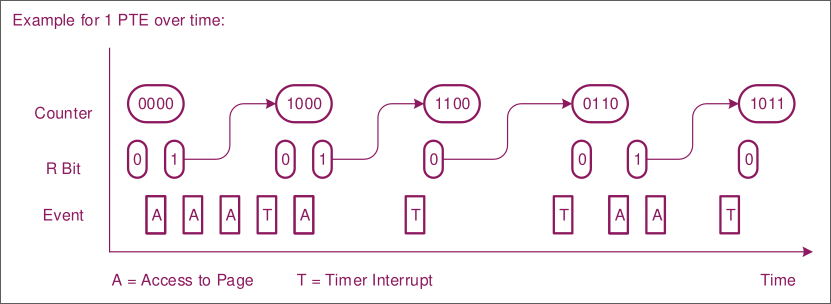
\includegraphics[scale=0.2]{2022-12-13-04_37_48.png}

\subsubsection{Working Set}
\textcolor{purple}{Uses page-fault interrupt. Chooses an interval T.}\newline
if A set at interrupt, set A to 0 and timestamp now.\newline
if A not set, check if timestamp is smaller than T:\newline
\textcolor{red}{If timestamp smaller than T, \textbf{page not in working set}}\newline
\textcolor{red}{If timestamp NOT smaller than T, \textbf{page in working set}}\newline
If page not in working set, page can be cleaned with a cleaning algorithm of choice, whenever needed.

\subsubsection{WS Clock}
Same as Working set with proper Clock instead of timestamping, iterates over clock at fault-interrupt.\newline
\textcolor{purple}{Same structure as Clock from second chance}

\end{multicols*}
\end{document}
